\part{Overview, background and setup}

\begin{frame}
    \partpage
\end{frame}

\begin{frame}
    \frametitle{Outline: Overview, background and setup}
    \tableofcontents[currentsection]
\end{frame}

\section{About the course}

\subsection{Who this course is for}

\begin{frame}{Who is this course for?}

People who have had a litte experience with Git, but want to use Git more
confidently and level up their skills.

\end{frame}

\subsection{Goals}

\begin{frame}
\frametitle{Course goals}

At the end of this course you should:

\begin{itemize}
    \item feel comfortable using Git
    \item know where to get further help, if necessary
    \item be able to use Git on private projects
    \item be able to collaborate with others online
\end{itemize}
\end{frame}

\begin{frame}
\frametitle{Course outline}
\begin{itemize}
    \item Introduction to Git and version control
    \item Supporting tools
    \item Using Git on your own
    \item General Git workflow
    \item Working with others
\end{itemize}
\end{frame}

% XXX: course flow as diagram

\subsection{Website and repository}
\begin{frame}
\frametitle{Course information}
\begin{itemize}
    \item Feedback most welcome!
    \item Slides are available on GitHub:\\
        {\footnotesize \url{https://github.com/paultcochrane/git\_course/}}
\end{itemize}
\end{frame}

\subsection{About me}
\begin{frame}
\frametitle{About me}
\begin{itemize}
    \item Physicist originally from New Zealand
    \item Have been involved in scientific computing and
        scientific software development in Australia and Germany.
    \item Am active in the Perl programming language community.
    \item Led the scientific computing group at the Regional Computing
        Centre for Lower Saxony.
    \item Was CTO at a startup in Bremen making polar shipping safer with
        data from space.
    \item Currently a freelance software developer developing
        and maintaining Python and Perl backend systems.
\end{itemize}
\end{frame}

\section{Version control systems}

\begin{frame}
\frametitle{What are Version Control Systems?}
\begin{itemize}
    \item A way to track changes\footnote[frame]{e.g.\ what, when, by whom,
        and why} to groups of files
    \item Most often used in software projects
    \item Most often used to track changes to text files (but not
        exclusively)
\end{itemize}
\end{frame}

\begin{frame}[fragile]
\frametitle{What are Version Control Systems?}
\begin{itemize}
    \item Akin to a time machine: one can return to previous states of a
        project
\end{itemize}
\begin{figure}
    \centerline{%
    \includegraphics[width=0.7\textwidth]{images/The_Delorian_William_Warby_flickr.pdf}}
        \caption{\tiny \emph{The Delorian}, by William Warby, Flickr:
    \url{https://www.flickr.com/photos/wwarby/9641216546/in/photostream/}}
\end{figure}
\end{frame}

\begin{frame}[fragile]
\frametitle{What are Version Control Systems?}
    \begin{itemize}
        \item Like a safety net: accidental file deletion isn't a catastrophe
    \end{itemize}
    \begin{figure}
        \centerline{%
            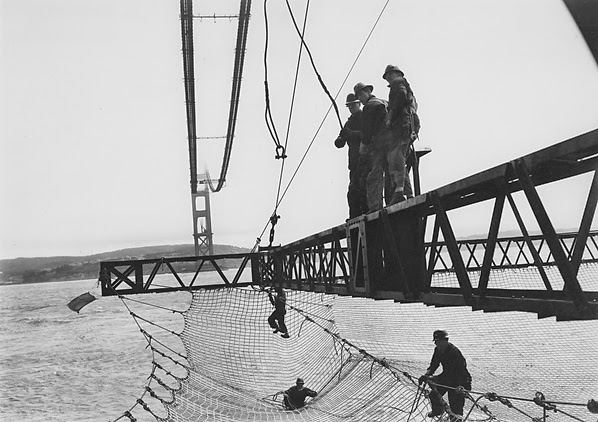
\includegraphics[height=0.65\textheight]{images/safety_net_golden_gate_bridge.jpg}}
            \caption{\tiny \url{https://todayinlaborhistory.wordpress.com/2015/01/05/january-5-1933/}}
    \end{figure}

\end{frame}

\begin{frame}[fragile]
\frametitle{What are Version Control Systems?}
    \begin{multicols}{2}
        \begin{itemize}
            \item Saved states are like anchor points in like rock climbing:
                one can fall a small distance without losing everything.
        \end{itemize}
        \begin{figure}
            \centerline{%
                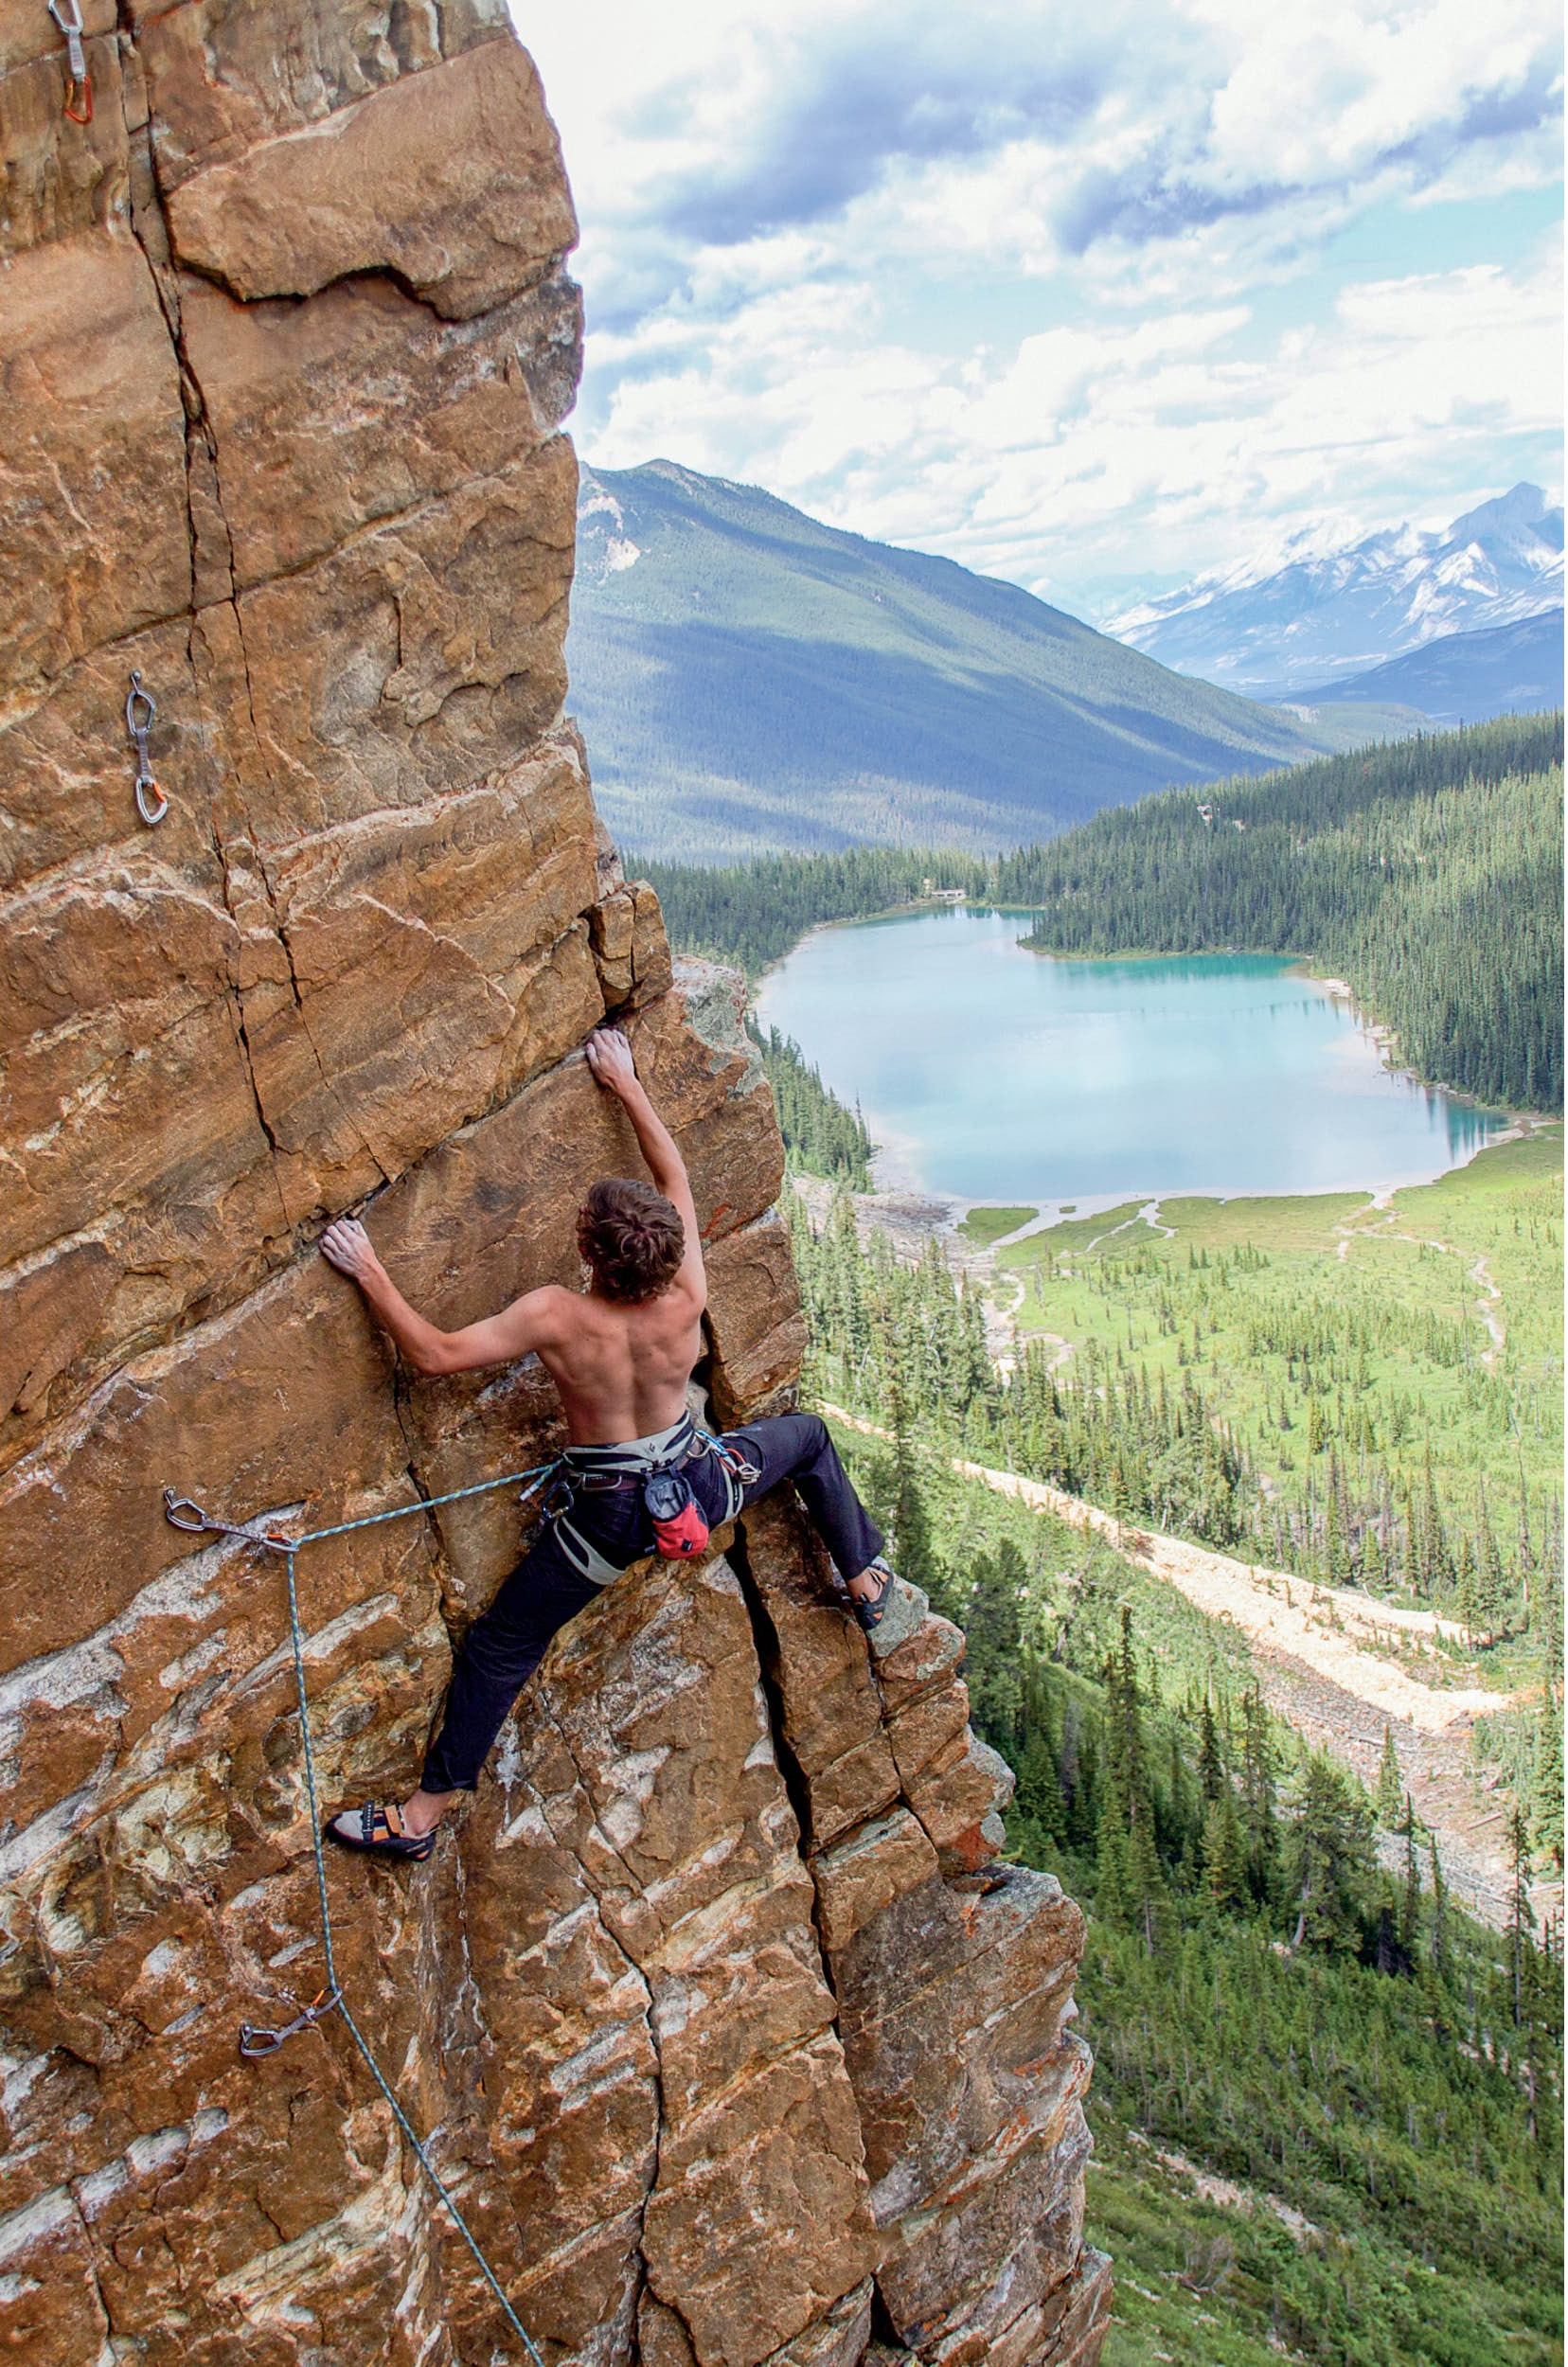
\includegraphics[height=0.8\textheight]{images/northern_exposure_jasper_rock_climbing.jpg}}
                \caption{\tiny by Fran\c{c}ois Laplante, \url{http://www.northernexposurejasper.com/}}
        \end{figure}
    \end{multicols}
\end{frame}

\begin{frame}[fragile]
\frametitle{Why use a Version Control System?}

Does this look familiar?

\inputminted{bash}{hand-rolled-version-control.txt}

This is better than nothing, however \ldots
\begin{itemize}
    \item what happened between the different versions?  And just as
        important: \emph{why}?
    \item which file is really the most current?
    \item what if \ttt{file.old} has the latest timestamp, i.e.\ it is the \emph{newest} file?
    \item can the differences between files tell us anything?
    \item why store \emph{nine} files when we really only need one?
\end{itemize}
\end{frame}

\begin{frame}
\frametitle{Why use a Version Control System?}
\begin{itemize}
    \item Version Control Systems (VCSs) help to tame this chaos
    \item Useful in detecting when bugs were introduced or fixed
    \item Used to save known states of a group of files and hence versions
        (releases) of a software project
    \item Can aid work on collaborative projects
\end{itemize}
\end{frame}

\begin{frame}
\frametitle{Who uses version control?}
\begin{itemize}
    \item Anyone wanting access to an old version of a document.
    \item Anyone working on a collaborative project.
    \item Anyone to whom such things have happened:
        \begin{itemize}
            \item ``It would be nice to have the version from 2 hours ago \ldots''
            \item ``I wrote that really well three days ago.  How did that
                go again?''
            \item ``Oh no!  I deleted the file!''
            \item ``Hrm, the application stopped working.  What changed in the
                last update?''
        \end{itemize}
\end{itemize}
\end{frame}

\begin{frame}
\frametitle{Where is version control used?}
    \begin{itemize}
    \item Software development
    \item Text and document processing/writing
        \begin{itemize}
            \item books
            \item scientific articles and talks
            \item letters
            \item documentation
            \item quotations and invoices
        \end{itemize}
    \item Graphic and web design
    \item System administration
        \begin{itemize}
            \item track changes to configuration files
            \item e.g.\ the tool \code{etckeeper} automates this process
        \end{itemize}
    \end{itemize}
\end{frame}

\begin{frame}
\frametitle{What should be kept under version control?}
\begin{itemize}
    \item Any kind of file that will be changed and where differences to
        previous states is of interest
    \item Mainly text files
        \begin{itemize}
        \item Program code, documentation
        \item Theses, dissertations
        \item Configuration files
        \end{itemize}
    \item Binary files also possible
        \begin{itemize}
        \item Graphics files: \code{.png}, \code{.tiff}
        \item Documents: \code{.odt}
        \end{itemize}
\end{itemize}
\end{frame}

\begin{frame}
\frametitle{What \emph{shouldn't} be kept under version control?}
\begin{itemize}
    \item Automatically generated files
        \begin{itemize}
            \item e.g.: \code{.o}, \code{.log}, \code{.pdf}, \code{.pyc}
        \end{itemize}
    \item Editor backup files
        \begin{itemize}
            \item e.g.: \code{file\~{}}, \code{file.bak}
        \end{itemize}
    \item Data files
        \begin{itemize}
            \item e.g.\ simulation input or output files
            \item are often static or change very seldom
            \item better kept on an FTP server or similar
        \end{itemize}
    \item Large files
        \begin{itemize}
            \item can make cloning a repository very slow
            \item cause unnecessary bloat
            \item if possible, avoid storing such files
            \item Git LFS can aid in keeping large files in version
                control without causing repository bloat
        \end{itemize}
\end{itemize}
\end{frame}

\section{Git history}

\begin{frame}
\frametitle{A short Git history}
\begin{itemize}
    \item Linux kernel development could use proprietary BitKeeper system
        free of charge
    \item The owners of BitKeeper changed the licensing conditions, which
        meant that it was no longer free for kernel developers to use
    \item This inspired Linus Torvalds to wrote his own system: Git
    \item Open source with a large developer community and an even larger
        user base.
\end{itemize}
\end{frame}

\begin{frame}
    \frametitle{Why use Git?}
    \begin{itemize}
        \item Supports distributed development
        \item Doesn't rely on network availability
        \item Scales to thousands of developers and millions of commits
        \item Fast!
        \item Repositories contain complete project history
        \item Lightweight branches
        \item Atomic operations
        \item Open source
        \item Free as in freedom
    \end{itemize}
\end{frame}

%%%%%%%%%%%%%%%%%%%%%%%%%%%%%%%%%%%%%%%%%%%%%%%%%%%%%%%%%%%%%%%%%%%%%%%%%%%%
\section{Installing Git}

\subsection{Graphical clients (GUIs)}

\begin{frame}
    \frametitle{Graphical Git clients}
    There are \emph{many} GUI clients to choose from.  E.g.:
\begin{itemize}
    \item SourceTree
        
\includegraphics[height=0.05\textheight]{images/Sourcetree-blue.pdf}
        \begin{itemize}
            \item \url{https://www.sourcetreeapp.com/}
            \item Windows, Mac
            \item A popular way to start using Git
            \item Blog article with more info:\\
                {\footnotesize \url{https://peateasea.de/installing-and-setting-up-sourcetree/}}
        \end{itemize}
    \item TortoiseGit
        
\includegraphics[height=0.05\textheight]{images/tgit_logo.pdf}
        \begin{itemize}
            \item \url{https://tortoisegit.org/}
            \item Windows
            \item Integrated into Windows Explorer
            \item Blog article with more info:\\
                {\footnotesize \url{https://peateasea.de/windows-git-installation/\#installing-tortoise-git}}
        \end{itemize}
\end{itemize}
\end{frame}

\begin{frame}
    \frametitle{Graphical Git clients (cont.)}
\begin{itemize}
    \item GitKraken
        
\includegraphics[height=0.05\textheight]{images/gitkraken-logo-dark-hz.png}
        \begin{itemize}
            \item \url{https://www.gitkraken.com/}
            \item Windows, Mac, Linux
            \item Another popular graphical client
            \item Restricted, free community edition.  More features in paid
                versions.
        \end{itemize}
    \item GitHub Desktop
        \begin{itemize}
            \item Official application: \url{https://github.com/apps/desktop}
            \item Windows, Mac
            \item Linux fork: \url{https://github.com/shiftkey/desktop}
            \item Tight integration with GitHub
        \end{itemize}
    \item Many more GUI clients can be found on the Git website:
        \begin{itemize}
            \item \url{https://git-scm.com/download/gui}
        \end{itemize}
    \end{itemize}
\end{frame}

\subsection{The command line interface (CLI)}

\begin{frame}
\frametitle{Use the command line!}
\begin{itemize}
    \item All graphical interfaces are essentially wrappers around Git's
        command line interface
    \item With the command line one can get futher and do more; the
        learning curve is steeper, but it's worth it.
    \item Hence, we will focus on the command line interface (CLI) from now
        on.
    \item E.g.\ bash, fish, zsh (on Linux/Unix); Powershell, Command (on
        Windows); iTerm, etc. (on MacOS)
    \item Behaviour is the same everywhere with the command line.
    \item Starting with a GUI is a good introduction, but the command line
        will take you further
\end{itemize}
    \blockquote[Hunt and Thomas, \emph{The Pragmatic Programmer}]
    {Gain familiarity with the shell, and you'll find your productivity soaring.}
\end{frame}


\begin{frame}
\frametitle{Installing Git (CLI options; Windows)}
\begin{itemize}
    \item download the installer from \url{https://git-scm.com/download/win}
    \item double click the downloaded \code{.exe} file and follow the
        installation instructions to install it
\end{itemize}
\end{frame}


\begin{frame}
\frametitle{Installing Git (CLI options; MacOS)}
\begin{itemize}
    \item download the installer from \url{https://git-scm.com/download/mac}
    \item double click the downloaded image file to install it
        % TODO: add installation screens to slides
\end{itemize}
\end{frame}


\begin{frame}[fragile]
\frametitle{Installing Git (CLI options; Linux/Unix)}
\begin{itemize}
    \item either via a package manager, e.g.:
\end{itemize}

\begin{lstlisting}
sudo apt install git  # Debian-based distributions
sudo yum install git  # RedHat-based distributions
\end{lstlisting}

\begin{itemize}
    \item or via the source code:
\end{itemize}

\begin{lstlisting}[
    breaklines=true,
    postbreak=\mbox{$\hookrightarrow$\space}]
wget https://mirrors.edge.kernel.org/pub/software/scm/git/git-<version>.tar.gz
tar -xvzf git-<version>.tar.gz
cd git-<version>
./configure
make
make test  # optional
sudo make install
\end{lstlisting}

\begin{itemize}
    \item more help is available on the Git Linux/Unix download page:
        \url{https://git-scm.com/download/linux}
\end{itemize}
\end{frame}

% vim: expandtab shiftwidth=4:

%%%%%%%%%%%%%%%%%%%%%%%%%%%%%%%%%%%%%%%%%%%%%%%%%%%%%%%%%%%%%%%%%%%%%%%%%%%%

\section{Tools}

\begin{frame}
\frametitle{Text editors}
\begin{itemize}
    \item We will be creating and editing text files, hence the need for a
        text editor.
    \item One of the fundamental tools of software development.
    \item Many options to choose from, including:
    \begin{itemize}
        \item \href{https://code.visualstudio.com/}{Visual Studio Code} (Windows, Mac, Linux)
        \item \href{https://notepad-plus-plus.org/}{Notepad++} (Windows)
        \item \href{https://www.sublimetext.com/}{Sublime text} (Windows, Mac, Linux)
        \item \href{https://www.vim.org/}{Vim} (Mac, Linux)
        \item \href{https://www.gnu.org/software/emacs/}{Emacs} (Mac, Linux)
    \end{itemize}
    \item The choice of editor is unimportant; what \emph{is} important is
        that you feel comfortable using yours.
\end{itemize}
\end{frame}

\section{Initial Git configuration}

\begin{frame}[fragile]{Warm up exercise}
    Before we start with the first demo, let's see what Git version we're
    running:
    \begin{minted}{shell}
        git --version
    \end{minted}
    Output:
    \begin{minted}{output}
        git version 2.39.5
    \end{minted}
    Note: your Git version is likely different to that shown above.
\end{frame}

\begin{frame}{A quick config demo}
    \begin{itemize}
        \item For Git to work 100\% from the get-go, we need to tell it who
            we are.
        \item But what happens if we don't tell Git who we are before using it?
        \item Let's be brave and run into a problem I know will appear so
            that you can avoid it in the future.
        \item Then we can discuss why Git needs this in the first place.
    \end{itemize}
\end{frame}

\begin{frame}[fragile]{A quick config demo}
    \begin{minted}{shell}
        mkdir who-are-you  # create example directory
        cd who-are-you  # change into new directory
        git init  # initialise new Git repository
        Initialized empty Git repository in /home/vagrant/who-are-you/.git/
        # create an example file with some content
        echo "# A project with an unknown author" > README.md
        git add README.md  # add the file to the staging area
        git commit README.md  # try to commit the change
    \end{minted}
\end{frame}

\begin{frame}[fragile]{A quick config demo}
    \begin{minted}{shell}
    Author identity unknown

    *** Please tell me who you are.

    Run

      git config --global user.email "you@example.com"
      git config --global user.name "Your Name"

    to set your account's default identity.
    Omit --global to set the identity only in this repository.\

    fatal: unable to auto-detect email address (got 'vagrant@bookworm.(none)')
    \end{minted}
\end{frame}

introduce git configuration; show git config --list output; mention
necessary initial configuration (name, email address) and explain why Git
requires this.  Show how to set this information.  Get participants to do
this on their own systems (or change the value if they have already set it).

Describe this as a demo, showing what goes wrong if one hasn't set up name
and email address before committing.

Main takeaway: you will run into problems when using Git.  Remain calm!

\begin{frame}[fragile]
    \frametitle{Detour: setting name and email metadata}
    If this is the first time you've installed Git, then one of the first
    things you need to do is to set your name and email address
    configuration metadata:
    \begin{minted}{shell}
        git config --global user.name "Your name"
        git config --global user.email "<username@example.com>"
    \end{minted}
\end{frame}

\begin{frame}[fragile]
    \frametitle{Exercise: explore \code{git config}}

    Open a terminal (or the Git-Bash shell in Windows) and enter the
    following commands:
    \begin{minted}{shell}
    git config
    git config --list
    git config --help
    \end{minted}

    \begin{itemize}
        \item describe the output of each command
        \item how does the output relate to the commands mentioned on the
            previous slide?
        \item if you need to find out detailed information about a command,
            what might you always be able to do?
    \end{itemize}
\end{frame}
